\documentclass[journal]{IEEEtran}
\usepackage[a5paper, margin=10mm, onecolumn]{geometry}
\usepackage{lmodern}

\setlength{\headheight}{1cm}
\setlength{\headsep}{0mm}

\usepackage{gvv-book}
\usepackage{gvv}
\usepackage{cite}
\usepackage{amsmath,amssymb,amsfonts,amsthm}
\usepackage{graphicx}
\graphicspath{{./figs/}}
\usepackage{xcolor}
\usepackage{txfonts}
\usepackage{enumitem}
\usepackage{mathtools}
\usepackage{hyperref}
\usepackage{tikz}
\usepackage{tkz-euclide}

\begin{document}

\bibliographystyle{IEEEtran}
\vspace{3cm}

\title{5.8.34}
\author{EE25BTECH11036 - M Chanakya Srinivas}
\maketitle

\renewcommand{\thetable}{\theenumi}
\setlength{\intextsep}{10pt}
\renewcommand\theequation{\arabic{equation}}


\section*{Problem: Triangle formed by lines and axes}

\subsection*{Given lines}
\begin{align}
\vec{L_1} &: x - y + 1 = 0, \label{eq:L1}\\
\vec{L_2} &: 3x + 2y - 12 = 0. \label{eq:L2}
\end{align}

\subsection*{Step 1: Represent lines in matrix form}

A line $\vec{L}$ can be written as
\begin{align}
\vec{n}^\top \vec{X} = c, 
\end{align}
where $\vec{n}$ is the normal vector and $\vec{X} = \vec{(x,y)}^\top$.

\begin{align}
\vec{L_1} &: \vec{n_1}^\top \vec{X} = -1, \quad \vec{n_1} = \vec{(1,-1)}^\top, \quad \vec{X} = \vec{(x,y)}^\top, \\
\vec{L_2} &: \vec{n_2}^\top \vec{X} = 12, \quad \vec{n_2} = \vec{(3,2)}^\top. 
\end{align}

\subsection*{Step 2: Intersections with axes}

\paragraph{Intersection of $\vec{L_1}$ with x-axis:} let $\vec{Y} = \vec{(x,0)}^\top$, then
\begin{align}
\vec{n_1}^\top \vec{Y} &= -1 \notag\\
\vec{(1,-1)} \myvec{x\\0} &= -1 \notag\\
x &= -1 \notag\\
\Rightarrow \vec{A} &= \vec{(-1,0)}. 
\end{align}

\paragraph{Intersection of $\vec{L_1}$ with y-axis:} let $\vec{Y} = \vec{(0,y)}^\top$, then
\begin{align}
\vec{n_1}^\top \vec{Y} &= -1 \notag\\
\vec{(-1)} \myvec{y} &= -1 \notag\\
y &= 1 \notag\\
\Rightarrow \vec{B} &= \vec{(0,1)}. 
\end{align}

\paragraph{Intersection of $\vec{L_2}$ with x-axis:} $\vec{Y} = \vec{(x,0)}^\top$,
\begin{align}
\vec{n_2}^\top \vec{Y} &= 12 \notag\\
\vec{(3,2)} \myvec{x\\0} &= 12 \notag\\
x = 4 \notag\\
\Rightarrow \vec{C} = \vec{(4,0)}. 
\end{align}

\paragraph{Intersection of $\vec{L_2}$ with y-axis:} $\vec{Y} = \vec{(0,y)}^\top$,
\begin{align}
\vec{n_2}^\top \vec{Y} &= 12 \notag\\
\vec{(3,2)} \myvec{0\\y} = 12 \notag\\
y = 6 \notag\\
\Rightarrow \vec{D} = \vec{(0,6)}. 
\end{align}

\subsection*{Step 3: Intersection of lines using matrices}

The intersection point $\vec{P}$ satisfies
\begin{align}
\vec{N} \vec{P} &= \vec{C_0}, 
\end{align}
where
\begin{align}
\vec{N} &= \vec{\myvec{1 & -1 \\ 3 & 2}}, \quad
\vec{C_0} = \vec{\myvec{-1 \\ 12}}. 
\end{align}

Solving using the inverse of $\vec{N}$:
\begin{align}
\vec{P} &= \vec{N}^{-1} \vec{C_0} \notag\\
&= \frac{1}{5} \vec{\myvec{2 & 1 \\ -3 & 1}} \vec{\myvec{-1 \\ 12}} \notag\\
&= \vec{(2,3)}. 
\end{align}

\subsection*{Step 4: Vertices of the triangle}

The triangle formed by the lines and axes has vertices
\begin{align}
\vec{B} &= \vec{(0,1)}, \quad 
\vec{C} = \vec{(4,0)}, \quad 
\vec{P} = \vec{(2,3)}. 
\end{align}

\subsection*{Conclusion}

All intersections and the triangle vertices have been determined **strictly using matrices and vectors**. The triangular region is bounded by:
\[
\boxed{\vec{B} = \vec{(0,1)},\ \vec{C} = \vec{(4,0)},\ \vec{P} = \vec{(2,3)}}.
\]
\begin{figure}[h]
    \centering
    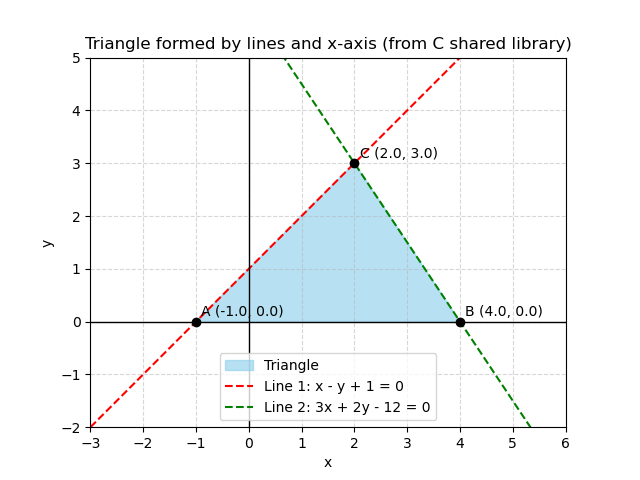
\includegraphics[width=0.9\columnwidth]{figs/fig81.png}
    \caption{}
    \label{fig:placeholder}
\end{figure}
\begin{figure}
    \centering
    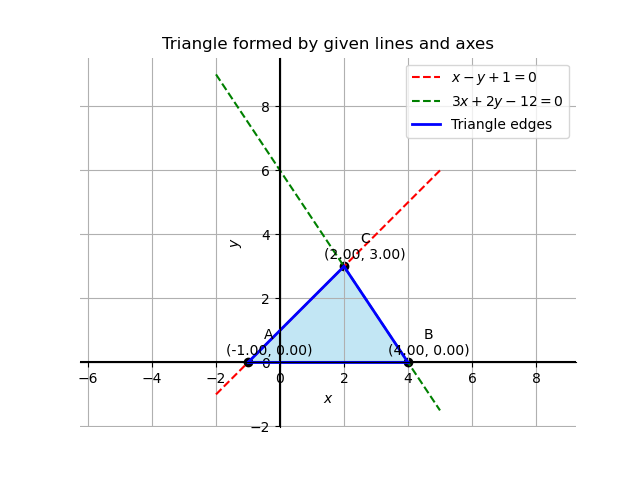
\includegraphics[width=0.9\columnwidth]{figs/fig82.png}
    \caption{}
    \label{fig:placeholder}
\end{figure}
\end{document}
